\documentclass{article}
\usepackage[utf8]{inputenc}
\usepackage{amsfonts}
\usepackage{amsmath}
\usepackage{graphicx}
\usepackage[a4paper, total={6in, 8in}]{geometry}
\usepackage{setspace}

\newcommand\tab[1][1cm]{\hspace*{#1}}
\onehalfspacing
\author{Frederic Becerril}

\begin{document}

\part*{Chapitre 2: Orthogonalité dans $\mathbb{R}^n$}

\section{\underline{Orthogonale d'un sous espace et projections orthogonales}}

\subsection{\underline{Orthogonal d'un sev:}}

Soit E un espace euclidien et V un sev de E \\
On note $V^\perp = \{x \in E \mbox{ tq } \forall v \in V, <x|v> = 0\}$ \\
Ce sont les éléments de E qui sont $\perp$ à \underline{tous} les éléments de V.

\paragraph{\underline{Proposition:}} Si $V = Vect\{a_1, \dots, a_k\}$ alors
$$x \in V^\perp \Leftrightarrow \forall 1 \leq i \leq k \tab[0.5cm] <x|a_i> = 0$$

\paragraph{\underline{Théorème:}} Si E est un espace euclidien (dimension finie) et V est un sev de E alors $V^\perp$ est un sev et
$$E = V \oplus V^\perp \tab \mbox{ de plus } (v^\perp)^\perp = V$$ 

\paragraph{\underline{Preuve:}}
\begin{itemize}
    \item Soit $\lambda,\; \mu \in \mathbb{R} \mbox{ et } x, y \in V^\perp$ alors:\\
$\forall v \in V \tab[0.5cm] <\lambda x + \mu y | v> = \lambda <x | v> + \mu <y | v> = 0$
Donc $V^\perp$ est stable par combinaisions linéaire et c'est donc un sev de E.
    \item V et $V^\perp$ sont toujours en somme directe.
Rappel de la définition. \\
$\forall x \in V + V^\perp \; \exists \mbox{ un unique couple } (x, y) de V \times V^\perp \mbox{ tel que } z = x + y$\\
Ce qui équivaut à $V \cap V^\perp = \{0\}$\\
Si $x \in V \cap V^\perp \tab x \in V^\perp \mbox{ et } \forall v \in V \tab <x|v> = 0$\\
d'où $<x|x> = 0 \mbox{ (en prenant v = x) } \Rightarrow x = 0 \mbox{ donc } V \cap V^\perp = \{0\}$
    \item Reste à montrer que $V + V^\perp = E$ Comme V et $V^\perp$ sont en somme directe, on a: \\
$dim(V + V^\perp) = dim V + dim V^\perp \mbox{ et } V + V^\perp \subset E$ de dimension n\\
Il suffit de montrer que $dim V^\perp = n - dim V$\\
car si $F \subset E$ et dim F = dim E, alors F = E

Si dim V = k, soit $\{u_1, \dots, u_k\}$ une base de V.\\
On sait qu'il existe $\{u_{k+1}, \dots, u_n\}$ tq $\{u_1, \dots, u_k, u_{k+1}, \dots, u_n\}$ soit une base de E

On orthonormalise par le procédé de Gram-Schmidt et on trouve un BON $\{e_1, \dots, e_n\}$ tq\\
$V = Vect\{e_1, \dots, e_k\} = Vect\{u_1, \dots, u_k\}$\\
Si $W = \{e_{k+1}, \dots, e_n\}$ alors par construction:
$$\forall x \in W, x \in V^\perp donc W \subset V^\perp$$
$$\mbox{et } n - k = dim(W) \leq dim(V^\perp)$$
Comme on a une somme directe et V $V \oplus V^\perp \subset E$
$$dim(V \oplus V^\perp) \leq dim E = n$$
$$\parallel \tab[2.5cm]$$
$$k + dim(V^\perp) \tab[2.3cm]$$
Donc $n - k \leq dim(V^\perp) \leq n - k$\\
On trouve donc vien que $W = V^\perp$ et $dim V^\perp = n - k$\\
Donc $V \oplus V^\perp = E$\\
C'est une façon de construire l'orthogonal
    \item Enfin on montre que $V \subset (V^\perp)^\perp$ et de même dimension
\end{itemize}

\paragraph{\underline{Remarque 1:}} Soit V un sous ensemble (pas un sev forcément) de E, alors on peut définir de la même façon $V^\perp$ et alors $V^\perp = (Vect V)^\perp$ est un sev

\paragraph{\underline{Remarque 2:}} Si E n'est pas de dimension finie alors on à encore $V + V^\perp = V \oplus V^\perp \mbox{ et } V^\perp$ sev mais pas forcément $V \oplus V^\perp = E$

\subsection{\underline{Exemples et calcul pratique}}

\subsubsection{\underline{Orthogonal d'un sev engendré par des vecteurs dans $\mathbb{R}^n$}}

Dans $\mathbb{R}^4$, soient
$$A = \begin{pmatrix}
    1\\
    0\\
    0\\
    1\\
\end{pmatrix} \mbox{ et } B = \begin{pmatrix}
    1\\
    2\\
    1\\
    0\\
\end{pmatrix} \mbox{ et } V = Vect\{A, B\} \mbox{ (dim 2)}$$

On trouve facilement les équations cartésiennes de $V^\perp$

$$\begin{pmatrix}
    x\\
    y\\
    z\\
    t\\
\end{pmatrix} = X \in V^\perp \Leftrightarrow
\left\{
    \begin{array}{ll}
        <X|A> = 0\\
        <X|B> = 0
    \end{array}
\right. \Leftrightarrow
\left\{
    \begin{array}{ll}
        x + t = 0\\
        x + 2y + z = 0
    \end{array}
\right.$$
Si on échalonne:
$$X \in V^\perp \Leftrightarrow \exists(z, t) \in \mathbb{R}^2 \mbox{ tq } X = \begin{pmatrix}
    -t\\
    \frac{-z}{2} + \frac{t}{2}\\
    z\\
    t\\
\end{pmatrix} = t \begin{pmatrix}
    -1\\
    \frac{1}{2}\\
    0\\
    1\\
\end{pmatrix} + z \begin{pmatrix}
    0\\
    -\frac{1}{2}\\
    1\\
    0\\
\end{pmatrix}$$

$$\mbox{d'où } V^\perp = Vect \left\{
    \begin{pmatrix}
        -1\\
        \frac{1}{2}\\
        0\\
        1\\
    \end{pmatrix}, \begin{pmatrix}
        0\\
        -\frac{1}{2}\\
        1\\
        0\\
    \end{pmatrix}
\right\}$$

On peut verifier ici que dim $V^\perp = 2$ et on pourrait même en donner une BON.\\
(On peut aussi trouver une BON de V facilement)

\subsubsection{\underline{Orthogonal d'un sev donné par des equations cartésiennes}}
Dans $\mathbb{R}^4$, si
$F = \left\{
    \begin{array}{ll}
        (x, y, z, t)^T \mbox{ tq }\; \begin{matrix}
            x + y + z + t = 0\\
            y + 2z + 3t = 0\\
        \end{matrix}
    \end{array}
\right\}$ soit $U = \begin{pmatrix}
    1\\
    1\\
    1\\
    1\\
\end{pmatrix}, V = \begin{pmatrix}
    0\\
    1\\
    2\\
    3\\
\end{pmatrix}$\\

$X \in F \Leftrightarrow <X|U> = 0 \mbox{ et } <X|V> = 0 \Leftrightarrow X \in \{U, V\}^\perp$\\
\tab[1.5cm] $\Leftrightarrow X \in Vect\{U, V\}^\perp$ d'où\\
F = $Vect\{U, V\}^\perp$ et donc $F^\perp = (Vect\{U, V\}^\perp)^\perp = Vect\{U, V\}$\\
On peut aussi orthonormaliser $\{u, v\}$ et on peut aussi trouver comme précédement des équations cart de $F^\perp$ en choisissant une base de F\\
$X \in F \Leftrightarrow X = (x, y, z, t)^T \mbox{ tq } \left\{
    \begin{matrix}
        x = -y -z -t\\
        y = -2z -3t\\
    \end{matrix}
\right.  \mbox{ ie } \left\{
    \begin{matrix}
        x = z + 2t\\
        y = -2z - 3t
    \end{matrix}
\right.$\\
d'où $F = Vect\left\{
    \begin{pmatrix}
        1\\
        -2\\
        1\\
        0\\
    \end{pmatrix}, \begin{pmatrix}
        2\\
        -3\\
        0\\
        1\\
    \end{pmatrix}
\right\}$

\newpage

\subsection{\underline{Projection et symetries orthogonales}}

\paragraph{\underline{Rappel:}} 
Soit E un espace vectoriel qui se décompose en somme directe\\
$E = F \oplus G$ (ie $E = F + G$ et $F \cap G = 0$)\\
Cela équivaut à dire que pour tout $x \in E$ il \underline{existe} un \underline{unique} $y \in F$ et $z \in G$ tels que $x = y + z$\\
On nomme $y = p(x)$ le projeté sur F parallèlement à G. Et $z = q(x)$ le projeté de x sur G parallèlement à F.\\
On montre alors que $P : E \rightarrow E$ et $q : E \rightarrow E$ sont bilinéaire, p + q = $id_E$ et $p \circ p = p$, $q \circ q = q$ (projections)\\


\paragraph{\underline{Définition:}} Soit E un espace euclidien et F un sous ev de E.\\
La projection orthogonale sur F est la projection sur F parallèlement à $F^\perp$ ($E = F \oplus F^\perp$), On la note $P_F$

\paragraph{\underline{Théorème:}} Si E euclidien et F est un sev de E
\begin{itemize}
    \item pour tout $x \in E, P_F(x)$ est l'unique vecteur de F tel que:
$$||x - P_F(x)|| = \underset{y \in F}{inf} ||x - y|| = d(x, F)$$
    \item Si $\{u_1, \dots, u_k\}$ est une BON de F alors.
$$P_F(x) = <x|u_1>u_1 + \dots + <x|u_k>u_k$$
\end{itemize}

\paragraph{\underline{Preuve:}} Soit $y \in F$
\begin{itemize}
    \item[] $||x - y||^2 = ||\underset{F^\perp}{\underbrace{x - P_F(x)}} + \underset{F}{\underbrace{P_F(x) - y}}||^2$ donc
    \item[] $||x - y||^2 = ||x - P_F(x)||^2 + ||P_F(x) - y||^2$
    \item[] $||x - y||^2 \geq ||x - P_F(x)||^2$ et est égal si $y = P_F(x)$
\end{itemize}

On remarque que $y = <x|u_1>u_1 + \dots + <x|u_k>u_k \in F$\\
si $z = x - y$ alors pour $1 \leq i \leq k \tab <z|u_i> = <x|u_i> - <y|u_i> = <x|u_i> - <x|u_i> = 0$\\
d'où $z \in Vect\{u_1, \dots, u_k\}^\perp = F^\perp \mbox{ donc } x = y + z \mbox{ et } y = P_F(x)$ 

\paragraph{\underline{Exemple pratique:}} si $x = \begin{pmatrix}
    1\\
    1\\
    1\\
    1\\
\end{pmatrix}$, calculer la distance de x à $Vect\left\{
    \begin{pmatrix}
        1\\
        1\\
        0\\
        0\\
    \end{pmatrix}, \begin{pmatrix}
        0\\
        1\\
        1\\
        0\\
    \end{pmatrix}
\right\}$ soit encore (au carré)
$$\underset{a,b \in R}{inf} (1 - a)^2 + (1 - a - b)^2 + (a - b)^2 + 1 \dots $$
Pour finir:\\
Si $E = F \oplus G$ et p est la projection sur F parallèlement à G, on a $s = 2p - id_E$ est la symétrie par rapport à F parallèlement à G\\
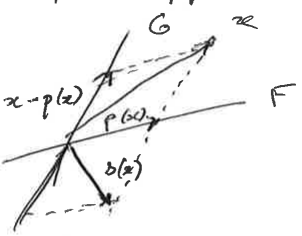
\includegraphics{images/image01.png} on a toujours $s \circ s = id_E$\\
Si $E = F \oplus F^\perp$ alors on parle de symetrie orthogonale et dans ce cas on a une formule dans une BON\\
pour tout $x \in E$



\begin{center}
    \begin{minipage}{0.50\textwidth}
        \begin{itemize}
            \item[$||s_F(x)||^2 =$]  $||P_F(x) + P_F(x) - x||^2$ 
            \item[$=$]  $||P_F(x)||^2 + ||P_F(x) - x||^2$ 
            \item[$=$]  $||P_F(x)|| + ||x - P_F(x)||^2 = ||x||^2$ 
        \end{itemize}
    \end{minipage}
\end{center}
C'est ce qu'on appelle une isométrie.

\end{document}